% !TEX root = ../../../main.tex
% 来源：中学数学实验教材·第三册（高中数学）
% 章节：函数及其图象 / 一次函数（线性函数）
% 原始文件：4.tex，行 1870-1880
% 类型：tikz
% ---
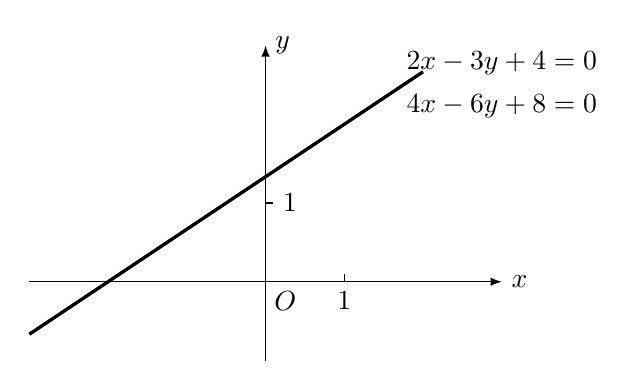
\begin{tikzpicture}[>=latex]
    \draw[->] (-3,0)--(3,0)node[right]{$x$};
    \draw[->] (0,-1)--(0,3)node[right]{$y$};
    \node at (.25,-.25){$O$};   
\draw[domain=-3:2, samples=10, very thick]plot (\x, {2*\x/3+4/3});
\node at (3,2.5)[below]{$4x-6y+8=0$};
\node at (3,2.5)[above]{$2x-3y+4=0$};
\draw (1,0)node[below]{1}--(1,.1);
\draw (0,1)--(.1,1)node[right]{1};

\end{tikzpicture}
